% options:
% thesis=B bachelor's thesis
% thesis=M master's thesis
% czech thesis in Czech language
% slovak thesis in Slovak language
% english thesis in English language
% hidelinks remove colour boxes around hyperlinks

\documentclass[thesis=B,czech]{FITthesis}[2012/06/26]

\usepackage[utf8]{inputenc}

% \usepackage[unicode]{hyperref}

\usepackage{graphicx} %graphics files inclusion
% \usepackage{amsmath} %advanced maths
% \usepackage{amssymb} %additional math symbols

\usepackage{dirtree} %directory tree visualisation

% % list of acronyms
% \usepackage[acronym,nonumberlist,toc,numberedsection=autolabel]{glossaries}
% \iflanguage{czech}{\renewcommand*{\acronymname}{Seznam pou{\v z}it{\' y}ch zkratek}}{}
% \makeglossaries

\newcommand{\tg}{\mathop{\mathrm{tg}}} %cesky tangens
\newcommand{\cotg}{\mathop{\mathrm{cotg}}} %cesky cotangens

% % % % % % % % % % % % % % % % % % % % % % % % % % % % % % 
% ODTUD DAL VSE ZMENTE
% % % % % % % % % % % % % % % % % % % % % % % % % % % % % % 

\department{Katedra \ldots (softwarového inženýrství)}
\title{ InfoWeb - Nástroj získávání informací z webů }
\authorGN{Jakub} %(křestní) jméno (jména) autora
\authorFN{Tuček} %příjmení autora
\authorWithDegrees{} %jméno autora včetně současných akademických titulů
\supervisor{Ing. Jiří Hunka}
\acknowledgements{Chtěl bych poděkovat za trpělivost vedoucímu, Ing. Jiřímu Hunkovi.}
\abstractCS{V~několika větách shrňte obsah a přínos této práce v~češtině. Po přečtení abstraktu
by se čtenář měl mít čtenář dost informací pro rozhodnutí, zda chce Vaši práci číst.}
\abstractEN{Sem doplňte ekvivalent abstraktu Vaší práce v~angličtině.}
\placeForDeclarationOfAuthenticity{V~Praze}
\declarationOfAuthenticityOption{4} %volba Prohlášení (číslo 1-6)
\keywordsCS{Nahraďte seznamem klíčových slov v češtině oddělených čárkou.}
\keywordsEN{Nahraďte seznamem klíčových slov v angličtině oddělených čárkou.}

\begin{document}

% \newacronym{CVUT}{{\v C}VUT}{{\v C}esk{\' e} vysok{\' e} u{\v c}en{\' i} technick{\' e} v Praze}
% \newacronym{FIT}{FIT}{Fakulta informa{\v c}n{\' i}ch technologi{\' i}}

\begin{introduction}
V předmětech BI-SP1 a BI-SP2 v prostředí FIT ČVUT byl realizován týmový projekt umožňující získávání informací z webů s primárním zaměřením na potřeby obchodů. Projekt řešil problém automatizace získávání dat z webů, jelikož stávající služby neposkytují veřejné rozhraní
nebo mají velkou chybovost dat.
\par
Práce pojednává o požadavcích internetových obchodů, které jsou především tvořeny nutností držet krok s trhem a sledovat vývoj cen
prodávaných produktů u konkurence.
\par
Cílem této práce je popsat požadavky internetových obchodů, stávající stav a možná řešení. Dále na základě těchto poznatků
zhodnotit vytvořené řešení a včetně korektnosti zvolených postupů navrhnout vylepšení. Ty implementovat, řádně vylepšení
otestovat a zhodnotit výsledný stav projektu.


\newpage

\newpage

\end{introduction}

\chapter{Cíl práce}

\section{Analytické cíle}

\begin{enumerate}  
\item Rešerše aktuálního stavu získávání dat pro potřeby
internetových obchodů
\item Analýza vzniklého řešení týmového projektu vzniklého v prostředí ČVUT FIT,
včetně důrazu na použité postupy při softwarovém vývoji
\item Návrh a zhodnocení implementovaných vylepšení
\end{enumerate}

\section{Praktické cíle}
\begin{enumerate}  
\item Implementace vylepšení systému
\end{enumerate}

\newpage


\chapter{Popis problematiky získávání informací z webů}

V této kapitole se budu nejprve zabývat samotnou problematikou získávání informací 
z webů s důrazem na internetové obchody.
Jelikož je tato problematika již řešena existujícími službami, je nejprve nutné služby zhodnotit a zanalyzovat jejich funkcionalitu.


\section{Problematika}
Získávání informací z webů je efektivní možnost jak získat databázi informací, které se na internetu vyskytují.
Tato činnost však stojí na problematice data získávat a uchovávat v potřebné struktuře, jelikož 
jinak z dat nejsme schopni vyčíst potřebné informace.
Vzhledem k specificitě dat, které jsou v kontextu činnosti zajímavá a dále kvůli unikátnosti webových stránek
není možné jednoznačně určit jednotný a zcela automatizovaný postup, jak data získat v požadovaném formátu.

\newpage

\section{Výběr dat}
Nejčastější řešení je kombinace automatizace a prvku lidské inteligence.
To je obvykle dosaženo roboty, kteří data stahují a lidské práce určující jaké informace nás ve stažených datech zajímají.
\par
Získávání informací ze stažených stránek lze poté zjednodušit na problematiku určení elementů v HTML, které jsou pro 
nás zajímavé.
Lokaci elementu v HTML se kterým je potřeba pracovat lze poté jednoznačně určit pomocí dvou možností:
\begin{enumerate}
\item XPath
\item CSS Selector
\end{enumerate}

\section{XML Path Language}
XML Path Language\cite{XPath} nazývaný zkráceně XPath je jazyk, který slouží k výběru elementu v dokumentu ve formátu XML\cite{XML} .
\par
XML chápeme jako jazyk popisující strukturu dat, které jsou strojově i lidsky čitelné.
HTML lze chápat jako strukturu podobnou XML, ačkoliv se přímo o XML dokument nejedná \cite{HTML}. HTML popisuje obsah dat pro prezentaci ve webovém prohlížeči pomocí předem definované struktury, které prohlížeče rozumí.
Díky této vlastnosti lze použít XPath pro definování cesty k prvku (a jeho obsahu),
který uchovává potřebnou informaci na webové stránce.
\par
\section{CSS Selector}
Jazyk CSS je používán pro vizuální popis prezentace webové stránky definované v HTML. Jazyk k určení prvků se kterými
chce pracovat používá selektory, které označují prvek v HTML. Jako selektor může být použit jak samotný název prvku,
tak vlastní definované třídy.\cite{CSS}
\par
Pomocí řetězení těchto selektorů jsme schopni jednoznačně získat element v HTML.

\newpage

\section{Současný stav řešení potřeb internetových obchodů}
I v kontextu malého trhu jako Česká republika se lze bavit o velké konkurenci na poli 
maloobchodů prodávající své zboží na internetu.
Internetové obchody potřebují monitorovat konkurenci a trh. Vzhledem k jejich zaměření je tedy nejvíce zajímají 
obchody prodávající stejné zboží. Potřebné informace o prodávaných produktů konkurencí 
se skládají z následujících hlavních atributů:

\begin{enumerate}
\item Název
\item Model
\item EAN
\item Cena
\item Inzerovaný název
\item Dostupnost
\end{enumerate}

\subsection{Srovnávače cen}

Data lze získat pomocí srovnávačů cen jako \textit{zbozi.cz}\cite{heureka} 
nebo \textit{heureka.cz}\cite{zbozi}. Problém u těchto spočívá v určení pro koncové zákazníky, kterým umožňuje
pro nalezení nejlepší ceny na trhu pro hledaný produkt. S tím souvisí to, že největší srovnávače cen neposkytují data nebo
rozhraní přes která by je bylo možné jednoduše získat.
\par
V rámci výzkumu pro bakalářskou práce jsem měl možnost nahlédnout do dat, které heuréka poskytuje obchodům. \cite{hunka}

Data obsahují následující informace:
\begin{itemize}
\item Informace o produktu - Segment, Kategorie, Jméno, ID, Výrobce, EAN, Item ID
\item Url na vlastním obchodu
\item Url na heuréce
\item Počet konkurence a popularita na trhu
\item Vlastní cena a pozice dle ní
\item Deset nejvyšších a nejnižších cen
\end{itemize}



První zásadní nedostatek zprávy z jmenovaného srovnávače se ukázal být logistický a to že obchod musí být označen \uv{Ověřeno zákazníky},
aby měl k datům přístup. Další nedostatek je, že data neobsahují žádná jména konkurenčních obchodů \cite{heureka-report}.
Vzhledem k povaze struktury a splatnosti generovaných dat je také nemožné ceny sledovat v časovém období.
Ostatní srovnávače mají údajně výstup velmi podobný nebo jako bylo výše řečeno data neposkytují. Díky tomu se ukázali
srovnávače jako nedostatečný zdroj dat.\cite{hunka}


\subsection{Existující služby}

Problematiku sledování trhu s důrazem na firemní klientelu, řeší aktuálně několik existujících služeb.
\par
Služby mají v zásadě velmi podobnou povahu služeb. Rámcově se jedná o porovnávání cen včetně historie na různých internetových
obchodem či na srovnávačích cen. Uživatel si zadá okruh či seznam produktů, buďto formou manuální či vstupem ze souboru, případně 
přímých napojením na e-shop. Následně je možné konkrétní data zobrazit v grafech označující vývoj cen, trendů či náhlých změn.
Dále umožňují externí výstup do souboru v dostupných formátech.
\par
Největší rozdíl služeb je zda jsou data získávána přímo z obchodů nebo ze srovnávačích. Další odlišností je 
možnost zda služba dokáže sledovat i zahraniční trh.
\par
Cena služeb se nejvíce odvíjí od počtu sledovaných produktů a četnosti aktualizací. Proto se měsíční platby mohou 
pohybovat od stovek korun po desítek tisíc korun.

\subsubsection{Price checking}

\subsubsection{Pricing intelligence}

\subsubsection{Sledování trhu}

\subsubsection{Pricebot}

\newpage

\subsubsection{Zahraniční nástroje}
Tyto nástroje jsou obecněji zaměřené a obvykle požadují od uživatele techničtější zaměření, 
jelikož je nutné přesně specifikovat kde, co a jak chce sledovat. Vzhledem k tomuto omezení
nejsou přímo pro provozovatele e-shopů vhodné kvůli nedostatečným technickým kapacitám a 
pro tuto práci důležité.
\par
Bodový seznam zahraničních nástrojů:

\begin{enumerate}
\item Screen scraper \cite{ScreenScraper}

  \begin{itemize}
    \item Webová služba
    \item procházení web skrz odkazy
    \item potvrzování formulářů
    \item využití interního vyhledávání
    \item export do širokého množství formátu souborů
    \item cena: \$549 - \$2,799 za měsíc
  \end{itemize}
  
\item Web extractor \cite{WebExtractor}

  \begin{itemize}
    \item Windows Aplikace
    \item procházení zadaných stránek
    \item hledání stránek pomocí klíčových slov
    \item export do csv formátu
    \item cena: \$99 - \$199 jednorázově
  \end{itemize}

\item Web Scraper \cite{WebScraper}

\end{enumerate}

\newpage

\chapter{Analýza týmového projektu}
V kapitole analýza týmového se budu věnovat řešení vytvořeného v rámci školní výuky na ČVUT FIT v akademickém roce 2015/16.
Nejprve popíšu cíl, který měl projekt za úkol řešit, jaké byly použité postupy při vývoji a mou roli v tomto projektu.

\section{Cíl týmového projektu}

V předmětech BI-SP1 a BI-SP2 byl realizován týmový projekt, v souladu s osnovami těchto předmětů byl nejdříve v BI-SP1 vytvořen návrh
systému a v BI-SP2 implementován.
\par
Hlavní funkcionalita systému spočívá v maximální možné míře automatizace získávání informací o produktech prodávaných konkurencí. Důraz je především kladem na optimalizaci počtu nutných lidských úkonů v rukách administrátora u kterého se předpokládá minimální technické vzdělání.
Jediná nutná problematika, co musí administrátor znát je parsování HTML stránek.
\par
Návrh popisuje rozdělení aplikace na část poskytující veškeré webový rozhraní a na část zpracovávající všechny interní procesy.
Vzhledem k požadavkům na škálovatelnost aplikace, druhá část se skládá z více samostatných menších služeb - modulů komunikující
spolu pomocí front. Díky tomu, že každý modul zajišťuje určitou funkcionalitu umožňující vytvářet více jeho instancí, je možné
procesy zpracovávat paralelně. 
Uživatelská a interní část spolu sdílejí data pomocí relační databáze\cite{DB}.
\par
%TODO - DOKUMENTACE - fronty atp.
\section{Webové rozhraní}
Webové rozhraní lze rozdělit na dvě části. Uživatelskou část obsahující množinu podstránek určených pouze pro konečné uživatele
služby. Uživatelská část umožňuje vytvořit kampaň. Kampaň je proces trvající určitý časový úsek, který sleduje vložené produkty u konkurence.
V těchto běžících kampaních má poté uživatel možnost uživatel vidět vizualizaci získaných dat, případně je umožněn export dat do formátu
csv nebo xlsx. Získaná data obsahují, kde se sledované produkty nacházejí a za jakou cenu se prodávají.
\par
Druhá část je určena pouze pro administrátory a slouží k monitorování kampaní uživatelů a řešení chyb, které systém není schopný vyřešit.
Chyby jsou typicky problémy s parsováním webových stránek, párování produktu ke stránce nebo potvrzení zda jsou získaná data validní.
\section{Interní část}
Interní část je rozdělena do samostatných modulů, které spolu komunikují pomocí front. Moduly jsou detailně popsány v následujících podsekcích.
\subsection{Manager}
Manager je hlavní modul, který jako jediný má možnost připojení přímo do sdílené databáze a jeho instance může existovat pouze jednou.
Manager má za úkol plánování práce pro ostatní části systému a zpracování vstupů a výstupů z front.
\subsection{Finder}
Finder je modul, který má za úkol získávat URL adresy internetových obchodů a na nich vyhledávat URL adresy vedoucí na požadované detaily produktů.
Detailem produktu je myšlena webová stránka, kde jsou obsažený podrobné informace o prodávaném produktu. Typicky je na takové stránce pouze jeden
produkt, případně odkazy na jiné detaily prodávaného zboží.
\subsubsection{DataProvider}
DataProvider je module, který zpracovává adresy vedoucí na detaily produktu. Zde existují čtyři hlavní větve možností zpracování požadavků.
Po stažení stránky, se z ní pokusí získat požadované
hodnoty. V případě neúspěchu odešle chybovou hlášku, v opačném případě data zanalyzuje korektnost získaných cen vůči historickým datům pokud
existují. Výsledek je poté odeslán k zpracování.  \uv{Managerem}

\begin{figure}\centering
 	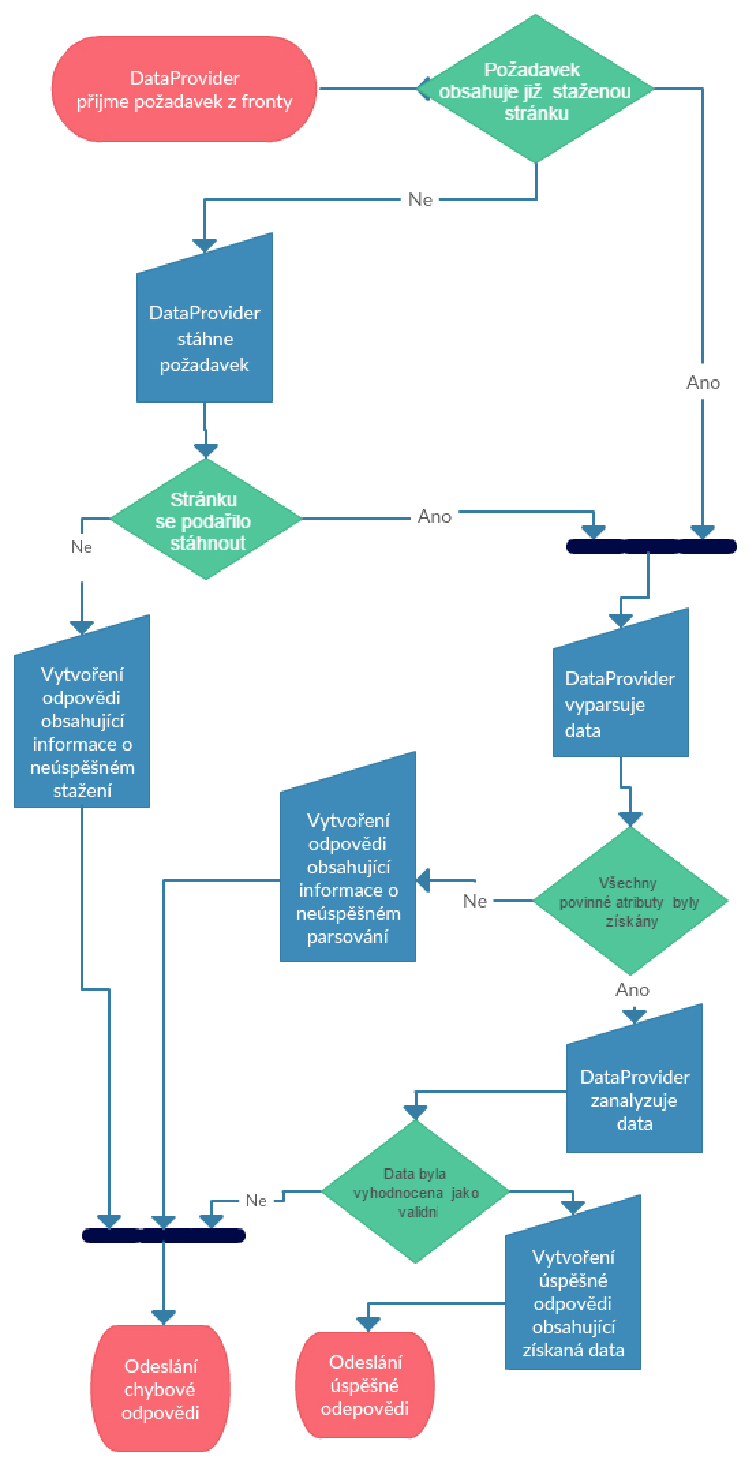
\includegraphics[width=0.8\textwidth]{resources/DataProvider-activity}
	\caption[DataProvider diagram]{Diagram zobrazující aktivity v DataProvider modulu}\label{fig:float}
\end{figure}

\chapter{Vývoj a implementace týmového projektu}

Nakonec rozeberu výslednou funkcionalitu oproti nárokům na plně funkční systém.
\section{Pojmy}

\subsection{Verzovací systém Git}
Git je pro sdílení jednotlivých verzí každého vývojáře, umožňující jednoduchý přehled nad rozpracovanými částmi každého vývojáře.
Úložiště systému se nazývá repositář, který obsahuje veškerý kód.
Základní jednotkou tvoří verze, které jsou postupně vytvářeny vývojáře po vytvoření každé malé funkcionality.
Verze jsou poté uchovávány v jednotlivých větví programu. Vedlejší větve slouží pro samotnou postupnou práci. 
Hlavní větve poté tento kód spojují.
Git také zajišťuje základní nástroje pro slučování kódu v případě spojování nebo slučovaní vedlejších větví do větví hlavních.
\subsection{Jednotkové a integrační testy}
Jednotkovými testy se rozumí sada kladných a záporných testů ověřující funkcionalitu jedné třídy.
Integrační testy pokrývají komunikaci více tříd.
\subsection{Statická analýza kódu}
Statická analýza kódu je analýza softwarového produktu, která běží bez spuštění samotné aplikace. Kontroluje 
pouze samotný kód. Označuje kritické konstrukce vedoucí k chybám nebo nedodržení programátorských konvencí daného
jazyka.
\subsection{Průběžná integrace}
Průběžnou integrací se rozumí sada nástrojů sloužící k rychlému nalezení případných chyb. Základní součástí je vzdálený repozitář, kde na 
základě každé jeho změny se vytváří nový build. Při buildu jsou poté spuštěny jednotkové a integrační testy.
Na jejich základě je poté možné zjistit případné chyby.

\section{Vývoj}
Vývoj byl rozdělen do 5 iterací, z nichž každá obsahovala 10 sprintů. Před začátkem vývoje byla rozdělena práce do těchto částí, 
s tím, že na konci každé iterace probíhala prezentace vyučujícímu. Každý sprint se skládal z jednotlivých
úkolů, které byly přiřazeny členům týmu. Stav úkolů byl uchováván na systému Redmine, ten umožňuje přehledné řízení projektu
a možnost sledování objevených chyb.
\par
Jako verzovací systém byl zvolen systém Git, zajišťován službou Gitlab. Gitlab umožňuje možnost uchovávat
repozitář na vzdáleném serveru a poskytuje webové rozhraní pro snadnou správu. Projekt byl v rámci repozitáře rozdělen na 4 části (větve):
\begin{itemize}
\item Master - hlavní větev uchovávající verze určené k nasazení na produkční server
\item Develop - vývojová větev obsahující aktuální stav vývoje
\item Feature - vedlejší větev vytvořená pro konkrétní úkol přidávající novou funkcionalitu
\item Fix - vedlejší větev určená pro úkoly opravující naleznou chybu
\end{itemize}
Jelikož přístup k přidání verze do Master a Develop měl pouze vedoucí projektu, musel být pro každou Feature a Fix větve
vytvořen požadavek o zařazení. Po kontrole vedoucím byl požadavek zařazen nebo vrácen k opravě.
\par
Na konci každé iterace byla poslední verze vždy označená ve verzovacím systému a poté prezentována vedoucímu.
Označení bylo zvoleno na základě pořadí iterace. 1. iterace je označena verzí \uv{0.1}.
\par
Pro vývoj se využil princip průběžné integrace. Každá verze byla zkompilována, otestována a zanalyzována na vzdáleném serveru.
Tyto činnosti zajišťovaly systém Jenkins a Gitlab. Jenkins aplikaci zkompiloval, spustil testy a statickou analýzu kódu 
zajištěnou systémem SonarQube. Výsledky poté publikoval ve svém webovém rozhraní a zároveň v rozhraní Gitlab.  
\section{Implementace}


\subsection{Webové rozhraní}
Webové rozhraní je implementováno v jazyce PHP verze 7. Základní kamenem aplikace zajišťuje aplikační rámec Nette. Nette
obsahuje nástroje pro automatickou správu závislostí, komunikaci s databází, vytváření bezpečných formulářů, zabezpečení
aplikace, šablonovací systém a rozhraní pro tvorbu jednotkových testů. Dále automaticky vynucuje MVC architekturu, která odděluje
prezenční a logickou vrstvu.

TODO = OBRAZEK MVC
%TODO - PIC	
\par
Snadnou správu závislostí umožňuje balíčkovací systém Composer. 
Na základě definujícího souboru, kde jsou uložený názvy požadovaných knihoven a jejich verze jsou automaticky 
stáhnuté z centrálního repositáře. Tím je mimo automatického stažení zajištěno, že každý člen týmu pracuje se stejnými verzemi knihoven.
\subsection{Interní část}
Interní část je implementována v jazyce Java verze 8. Kompilaci, spouštění testů a správu závislostí zajišťuje Gradle.
Gradle je nástroj sloužící k automatickému sestavení aplikace. Umožňuje správu závislostí, které stahuje z centrálního repositáře. V rámci sestavení lze pustit testy, včetně přídavných doplňků. Projekt používá
doplněk Cobertura, který na základě spuštěné testovací sady vytváří zprávu obsahující pokrytí větví programu.
Díky tomu lze jednoduše zjistit jaké větve aplikace nejsou otestované.
\par
Aplikace je rozdělena do nezávislých modulů běžící jako služby. Jednotlivé moduly spolu komunikují
pomocí posílání zpráv definovaných front. Komunikaci zajišťuje systém RabbitMQ Server implementovaný v jazyce Erlang. Zprávy jsou serializovatelné objekty, jejichž definice je sdílena napříč všemi moduly.
Serializace představuje proces, kdy je objekt serializovaný do posloupnosti bitů, které je poté
možné poslat jako zpráva. Vzhledem k sdílené podobě objektu je poté možné na druhé straně
objekt deserializovat zpět do Java objektu.

\par
Použité knihovny:
\begin{itemize}
\item Google Guice - automatická správa závislostí
\item Hibernate - objektově relační zobrazení databázových entit a práce s nimi
\item Apache Commons - pomocné knihovny pro práci s řetězcemi a soubory
\item RabbitMQ - zajišťuje komunikaci s frontami
\end{itemize}

\section{Má role}

\chapter{Zhodnocení týmového projektu}
Pro nutnost návaznosti na kapitolu o vylepšeních je nejprve nutné uvést v jakém kontextu jsou vylepšení navrhovány. K tomu je třeba
popsat výsledný stav projektu a jeho funkcionalitu. 

\section{Pojmy}

\subsection{JSON}
JSON označuje specifikaci formátu pro výměnu dat\cite{JSON}. Jedná se o formát, který je čitelný jak pro lidské oko tak pro stroj\cite{JSON} a jeho zpracování je implementováno pro velké množství programovacích jazyků\cite{JSON-impl}. Základní stavební jednotkou
tvoří kolekce párů klíč a hodnotu spolu se seřazeným polem hodnot.

\subsection{Web API}
Rozhraní, které na definovaný HTTP dotaz vrací data. Ty jsou standardně vracena ve formátech JSON nebo XML.

\section{Stav}
Ačkoliv stav projektu odpovídal nárokům na úspěšné odevzdání nebyla dosažena implementace všech procesů, aby byla umožněno reálně
použití systému.
\par
Odevzdávaný stav obsahoval funkční webové rozhraní, které se skládalo ze základní funkcionality pro uživatele a pro administrátory.
Část pro administrátory obsahovala správu uživatelů, možnost parsování stránek, evidenci známých obchodů a produktů či sledování
chyb vzniklých v interní části.
Uživatelská část umožňovala správu a vytvoření kampaně či kampaní. Implementace kampaní pak splňovala návrh z analytické částí,
která byla zmíněna výše.
Na žádost jiného týmu jsme také vytvořili REST rozhraní, poskytující získané ceny pro daný produktu.
\par
Interní část byla schopná pracovat pouze na základě dříve uložených url adres vedoucí detaily produktů. 
Manager dokázal zjistit vybrat produkty, které jsou v aktivní kampani a je třeba je aktualizovat.
Na základě výsledků poté vybral potřeba data odeslal požadavek pomocí pro zpracování do DataProvideru. Ten na základě obdržených dat stránku vyparsoval a zanalyzoval výsledek vůči historickým datům
a informacích o produktu. Analýza se především skládala z kontrol velkých výkyvů cen a rozdílných identifikátorů produktu.
V případě, že požadavek neobsahoval šablonu pro vyparsování nebo byl výsledek označen jako chybný, byla odeslána chyba
zpět do Manageru. Manager výsledek korektně a uložil pro zobrazení ve webovém rozhraní, ať už se jednalo o chybu
nebo nalezení ceny.
\par
Byla také obsažena detekce opravených chyb, díky kterému Manager poznal, že může pokračovat v práci hledání cen.

\subsection{Nedostatky}
Vytvořené řešení obsahovalo spoustu nedostatků, které je třeba v rámci této práce detekovat a ty nejdůležitější se pokusit opravit.
První zásadní problém bylo neefektivní chování komunikace modulu Manager s ProductProviderem. V rámci testování jsem zjistil, že v 
případě chyby při parsování stránky je stažené HTML odesláno pro znovupoužití, tak se po opravení parsovací šablony stažené HTML
nepoužije a detail je tak opětovně stažen. V případě chyb při analyzování, vznikal problém, že pro administrátora objevovali 
po jednou, což značně zhoršovalo efektivitu práce a celkovou uživatelskou přívětivost. Podobný případ se vyskytoval při neexistenci 
parsovací šablony. Systém totiž odeslal požadavek pro všechny uložené adresy na obchodu, ačkoliv šablona neexistovala. To vyústilo
ve vytvoření mnoho chyb, které musel administrátor všechny vyřešit.
\par
Druhy zásadní problém byla pouze částečná implementace modulu Finder u kterého byla funkcionalita ověřena pouze pomocí jednotkových
testů a modul jako celek nebyl zapojen do systému. Neexistovalo tedy rozhraní pro práci s frontami, ani část zajišťující vytváření
požadavků. K tomu je spojený celý proces párování detailu produktu.

\chapter{Návrh na vylepšení}
TODO

\chapter{Realizace vylepšení}

\chapter{Zhodnocení provedených vylepšení}
TODO
\section{Analýza nového řešení}
TODO


\chapter{Realizace}

\section{Způsob realizace stávajícího řešení}
TODO
\section{Implementace vylepšení}
TODO

\begin{conclusion}
	%sem napište závěr Vaší práce
\end{conclusion}

\bibliographystyle{csn690}

\bibliography{mybibliografy}

\appendix
\chapter{Seznam použitých zkratek}
% \printglossaries
\begin{description}
	\item[EAN] European Article Number
	\item[XML] Extensible markup language
	\item[HTML] Hypertext Markup Language
	\item[CSS] Cascading style sheets
	\item[JSON] JavaScript Object Notation
	\item[HTTP] Hypertext Transfer Protocol
\end{description}


% % % % % % % % % % % % % % % % % % % % % % % % % % % % 
% % Tuto kapitolu z výsledné práce ODSTRAŇTE.
% % % % % % % % % % % % % % % % % % % % % % % % % % % % 
% 
% \chapter{Návod k~použití této šablony}
% 
% Tento dokument slouží jako základ pro napsání závěrečné práce na Fakultě informačních technologií ČVUT v~Praze.
% 
% \section{Výběr základu}
% 
% Vyberte si šablonu podle druhu práce (bakalářská, diplomová), jazyka (čeština, angličtina) a kódování (ASCII, \mbox{UTF-8}, \mbox{ISO-8859-2} neboli latin2 a nebo \mbox{Windows-1250}). 
% 
% V~české variantě naleznete šablony v~souborech pojmenovaných ve formátu práce\_kódování.tex. Typ může být:
% \begin{description}
% 	\item[BP] bakalářská práce,
% 	\item[DP] diplomová (magisterská) práce.
% \end{description}
% Kódování, ve kterém chcete psát, může být:
% \begin{description}
% 	\item[UTF-8] kódování Unicode,
% 	\item[ISO-8859-2] latin2,
% 	\item[Windows-1250] znaková sada 1250 Windows.
% \end{description}
% V~případě nejistoty ohledně kódování doporučujeme následující postup:
% \begin{enumerate}
% 	\item Otevřete šablony pro kódování UTF-8 v~editoru prostého textu, který chcete pro psaní práce použít -- pokud můžete texty s~diakritikou normálně přečíst, použijte tuto šablonu.
% 	\item V~opačném případě postupujte dále podle toho, jaký operační systém používáte:
% 	\begin{itemize}
% 		\item v~případě Windows použijte šablonu pro kódování \mbox{Windows-1250},
% 		\item jinak zkuste použít šablonu pro kódování \mbox{ISO-8859-2}.
% 	\end{itemize}
% \end{enumerate}
% 
% 
% V~anglické variantě jsou šablony pojmenované podle typu práce, možnosti jsou:
% \begin{description}
% 	\item[bachelors] bakalářská práce,
% 	\item[masters] diplomová (magisterská) práce.
% \end{description}
% 
% \section{Použití šablony}
% 
% Šablona je určena pro zpracování systémem \LaTeXe{}. Text je možné psát v~textovém editoru jako prostý text, lze však také využít specializovaný editor pro \LaTeX{}, např. Kile.
% 
% Pro získání tisknutelného výstupu z~takto vytvořeného souboru použijte příkaz \verb|pdflatex|, kterému předáte cestu k~souboru jako parametr. Vhodný editor pro \LaTeX{} toto udělá za Vás. \verb|pdfcslatex| ani \verb|cslatex| \emph{nebudou} s~těmito šablonami fungovat.
% 
% Více informací o~použití systému \LaTeX{} najdete např. v~\cite{wikilatex}.
% 
% \subsection{Typografie}
% 
% Při psaní dodržujte typografické konvence zvoleného jazyka. České \uv{uvozovky} zapisujte použitím příkazu \verb|\uv|, kterému v~parametru předáte text, jenž má být v~uvozovkách. Anglické otevírací uvozovky se v~\LaTeX{}u zadávají jako dva zpětné apostrofy, uzavírací uvozovky jako dva apostrofy. Často chybně uváděný symbol "{} (palce) nemá s~uvozovkami nic společného.
% 
% Dále je třeba zabránit zalomení řádky mezi některými slovy, v~češtině např. za jednopísmennými předložkami a spojkami (vyjma \uv{a}). To docílíte vložením pružné nezalomitelné mezery -- znakem \texttt{\textasciitilde}. V~tomto případě to není třeba dělat ručně, lze použít program \verb|vlna|.
% 
% Více o~typografii viz \cite{kobltypo}.
% 
% \subsection{Obrázky}
% 
% Pro umožnění vkládání obrázků je vhodné použít balíček \verb|graphicx|, samotné vložení se provede příkazem \verb|\includegraphics|. Takto je možné vkládat obrázky ve formátu PDF, PNG a JPEG jestliže používáte pdf\LaTeX{} nebo ve formátu EPS jestliže používáte \LaTeX{}. Doporučujeme preferovat vektorové obrázky před rastrovými (vyjma fotografií).
% 
% \subsubsection{Získání vhodného formátu}
% 
% Pro získání vektorových formátů PDF nebo EPS z~jiných lze použít některý z~vektorových grafických editorů. Pro převod rastrového obrázku na vektorový lze použít rasterizaci, kterou mnohé editory zvládají (např. Inkscape). Pro konverze lze použít též nástroje pro dávkové zpracování běžně dodávané s~\LaTeX{}em, např. \verb|epstopdf|.
% 
% \subsubsection{Plovoucí prostředí}
% 
% Příkazem \verb|\includegraphics| lze obrázky vkládat přímo, doporučujeme však použít plovoucí prostředí, konkrétně \verb|figure|. Například obrázek \ref{fig:float} byl vložen tímto způsobem. Vůbec přitom nevadí, když je obrázek umístěn jinde, než bylo původně zamýšleno -- je tomu tak hlavně kvůli dodržení typografických konvencí. Namísto vynucování konkrétní pozice obrázku doporučujeme používat odkazování z~textu (dvojice příkazů \verb|\label| a \verb|\ref|).
% 
% \begin{figure}\centering
% 	
\includegraphics[width=0.5\textwidth, angle=30]{cvut-logo-bw}
% 	\caption[Příklad obrázku]{Ukázkový obrázek v~plovoucím prostředí}\label{fig:float}
% \end{figure}
% 
% \subsubsection{Verze obrázků}
% 
% % Gnuplot BW i barevně
% Může se hodit mít více verzí stejného obrázku, např. pro barevný či černobílý tisk a nebo pro prezentaci. S~pomocí některých nástrojů na generování grafiky je to snadné.
% 
% Máte-li například graf vytvořený v programu Gnuplot, můžete jeho černobílou variantu (viz obr. \ref{fig:gnuplot-bw}) vytvořit parametrem \verb|monochrome dashed| příkazu \verb|set term|. Barevnou variantu (viz obr. \ref{fig:gnuplot-col}) vhodnou na prezentace lze vytvořit parametrem \verb|colour solid|.
% 
% \begin{figure}\centering
% 	\includegraphics{gnuplot-bw}
% 	\caption{Černobílá varianta obrázku generovaného programem Gnuplot}\label{fig:gnuplot-bw}
% \end{figure}
% 
% \begin{figure}\centering
% 	\includegraphics{gnuplot-col}
% 	\caption{Barevná varianta obrázku generovaného programem Gnuplot}\label{fig:gnuplot-col}
% \end{figure}
% 
% 
% \subsection{Tabulky}
% 
% Tabulky lze zadávat různě, např. v~prostředí \verb|tabular|, avšak pro jejich vkládání platí to samé, co pro obrázky -- použijte plovoucí prostředí, v~tomto případě \verb|table|. Například tabulka \ref{tab:matematika} byla vložena tímto způsobem.
% 
% \begin{table}\centering
% 	\caption[Příklad tabulky]{Zadávání matematiky}\label{tab:matematika}
% 	\begin{tabular}{|l|l|c|c|}\hline
% 		Typ		& Prostředí		& \LaTeX{}ovská zkratka	& \TeX{}ovská zkratka	\tabularnewline \hline \hline
% 		Text		& \verb|math|		& \verb|\(...\)|	& \verb|$...$|		\tabularnewline \hline
% 		Displayed	& \verb|displaymath|	& \verb|\[...\]|	& \verb|$$...$$|	\tabularnewline \hline
% 	\end{tabular}
% \end{table}
% 
% % % % % % % % % % % % % % % % % % % % % % % % % % % % 

\chapter{Obsah přiloženého CD}

%upravte podle skutecnosti

\begin{figure}
	\dirtree{%
		.1 readme.txt\DTcomment{stručný popis obsahu CD}.
		.1 exe\DTcomment{adresář se spustitelnou formou implementace}.
		.1 src.
		.2 impl\DTcomment{zdrojové kódy implementace}.
		.2 thesis\DTcomment{zdrojová forma práce ve formátu \LaTeX{}}.
		.1 text\DTcomment{text práce}.
		.2 thesis.pdf\DTcomment{text práce ve formátu PDF}.
		.2 thesis.ps\DTcomment{text práce ve formátu PS}.
	}
\end{figure}

\end{document}
